\documentclass{beamer}

\usepackage{amsmath, amssymb}
%\usepackage[utf8]{inputenc}
\usepackage{zxjatype}
\usepackage[ipaex]{zxjafont}
\usepackage{mymacro}
\usepackage{booktabs}
\usepackage{array}
\usepackage{colortbl}
\usetikzlibrary{decorations.pathreplacing}

\usefonttheme{professionalfonts}
\setbeamertemplate{navigation symbols}{}

% --- page number ---
\setbeamertemplate{footline}{%
	\raisebox{10pt}{\makebox[\paperwidth]{\hfill\makebox[7em]{\normalsize\texttt{\insertframenumber/\inserttotalframenumber}}}}%
}

% Presenter's note
% \setbeameroption{show notes on second screen}

% Pictures are looked up in these folders, so \includegraphics needs only the file name
\graphicspath{{pics/}{figures/}}

\title{QuantHarness: Price-Driven Multi-Agent LLMs for High-Frequency Trading}
\subtitle{Fei Xiong, Xiang Zhang, Aosong Feng, Siqi Sun, Chenyu You}
\author{Paper review by Vasilisa Golikova}
\date{October 22, 2026}

\begin{document}

    \begin{frame}[plain]
        \maketitle
    \end{frame}

    \begin{frame}{Motivation and Research Question}
        \footnotesize
        Most LLM trading frameworks use text data for making decisions. QuantHarness reads only prices.

        \vspace{1em}
        {\renewcommand{\arraystretch}{1.5}
        \begin{tabular}{@{}>{\raggedright\arraybackslash}p{0.17\linewidth}>{\raggedright\arraybackslash}p{0.38\linewidth}>{\raggedright\arraybackslash}p{0.37\linewidth}@{}}
            \toprule
            & \textbf{Most LLM trading frameworks} & \textbf{QuantHarness} \\
            \midrule
            \textbf{Input} & News, social media, earnings reports & Price candles only (OHLC) \\
            \textbf{Horizon} & Long-term & The next 3 candles of 1h or 4h bars \\
            \textbf{Signal} & Lags the price, and is noisy, unstructured and hard to verify & Available as soon as a candle closes, and structured \\
            \bottomrule
        \end{tabular}\par}

        \vspace{1.5em}
        \colorbox{blue!8}{\parbox{\dimexpr\linewidth-2\fboxsep}{\small\vspace{0.3em}\textbf{Research question:} can LLM agents that only see price data predict short-term direction better than simple baselines?\vspace{0.3em}}}
    \end{frame}

    \begin{frame}{QuantHarness Architecture}
        
        \begin{itemize}
        \item QuantHarness is a collaborative framework for low-latency market decision-making which operates solely on price-derived market signals.

        \item In the code, the system splits trading into four specialized agents: IndicatorAgent, PatternAgent, TrendAgent, and DecisionAgent.
   
        \end{itemize}

        \centering
        \includegraphics[width=0.85\linewidth, trim=0 1060 0 680, clip]{merge.jpg}

        {\footnotesize The paper's RiskAgent (Fig.~2) turns the three reports into a risk--reward setup; in the code, the DecisionAgent does this\par}

    \end{frame}

    \begin{frame}{Indicator and Pattern}
        \begin{columns}[c]
            \begin{column}{0.36\linewidth}
                \footnotesize
                \textbf{IndicatorAgent}
                \begin{itemize}
                    \item Computes RSI, MACD, RoC, Stochastic, Williams \%R on the last 45 candles
                    \item Writes a short momentum report
                \end{itemize}
            \end{column}
            \begin{column}{0.64\linewidth}
                \includegraphics[width=\linewidth, trim=990 1670 1148 1102, clip]{indicator.jpg}

                {\centering\scriptsize Thresholds turn indicators into signals, e.g.\ RSI above 70 is bearish, below 30 bullish (paper, Fig.~1)\par}
            \end{column}
        \end{columns}
        \vspace{1.5em}
        \begin{columns}[c]
            \begin{column}{0.36\linewidth}
                \footnotesize
                \textbf{PatternAgent}
                \begin{itemize}
                    \item Gets a candlestick chart of the same candles
                    \item Picks the closest of 16 named patterns
                \end{itemize}
            \end{column}
            \begin{column}{0.64\linewidth}
                \includegraphics[width=\linewidth, trim=1043 1296 1126 1956, clip]{pattern.jpg}

                {\centering\scriptsize A sketch of the price moves is matched against a library of patterns, here a V-shaped reversal (paper, Fig.~1)\par}
            \end{column}
        \end{columns}
    \end{frame}


    \begin{frame}{Trend and Decision}
        \begin{columns}[c]
            \begin{column}{0.36\linewidth}
                \footnotesize
                \textbf{TrendAgent}
                \begin{itemize}
                    \item Gets the candles with fitted support and resistance lines
                    \item Calls the short-term trend upward, downward or sideways
                \end{itemize}
            \end{column}
            \begin{column}{0.64\linewidth}
                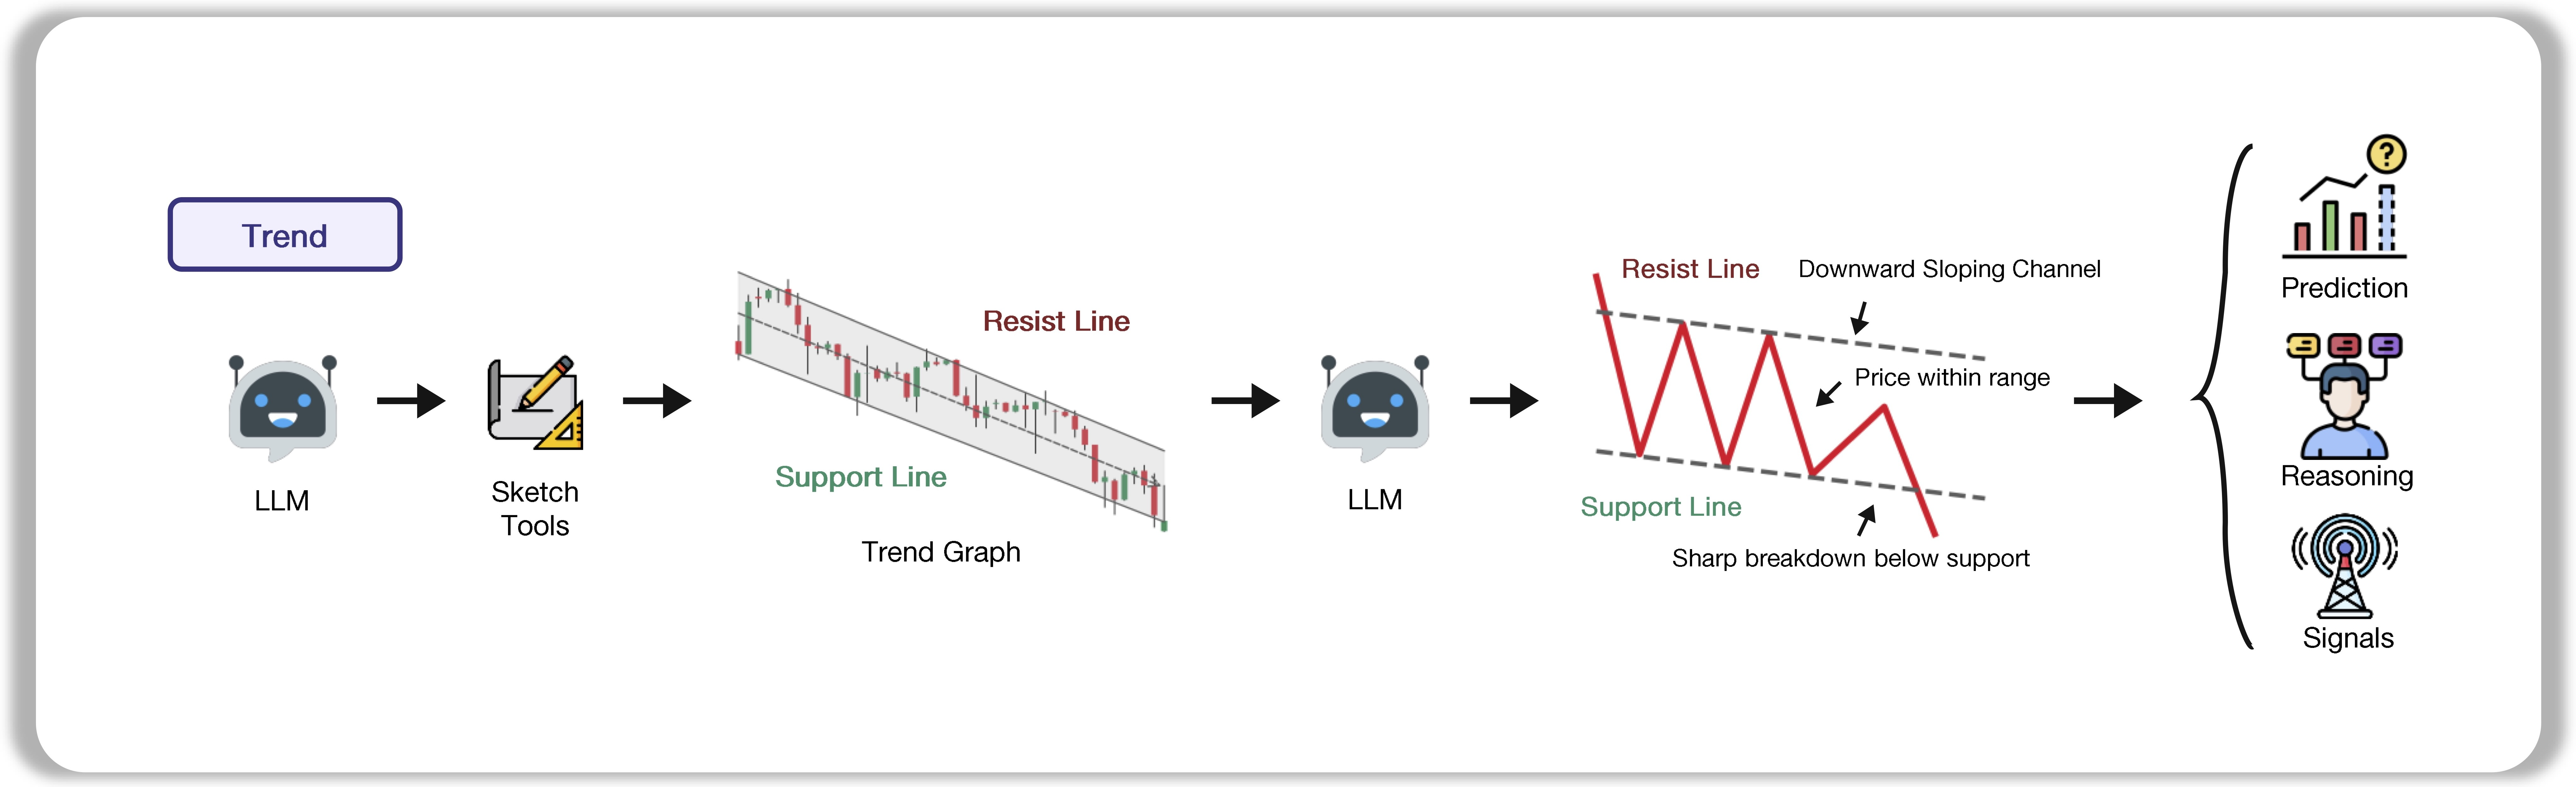
\includegraphics[width=\linewidth]{trend.jpg}

                {\centering\scriptsize A downward channel that breaks below support is read as bearish (paper, Fig.~1)\par}
            \end{column}
        \end{columns}
        \vspace{0.8em}
        \begin{columns}[c]
            \begin{column}{0.36\linewidth}
                \footnotesize
                \textbf{DecisionAgent}
                \begin{itemize}
                    \item Combines the three reports
                    \item Outputs LONG or SHORT with a justification and a risk--reward ratio
                \end{itemize}
            \end{column}
            \begin{column}{0.64\linewidth}
                \includegraphics[width=\linewidth, trim=382 2552 380 187, clip]{decision.jpg}

                {\centering\scriptsize Bullish evidence from the three reports becomes a LONG order with its justification (paper, Fig.~3)\par}
            \end{column}
        \end{columns}

        \vspace{0.6em}
        \colorbox{blue!8}{\parbox{\dimexpr\linewidth-2\fboxsep}{\scriptsize\textbf{Note:} the paper describes a separate RiskAgent for stop-loss and take-profit; in the code it is just one line of the DecisionAgent prompt asking for the risk--reward ratio.}}
    \end{frame}


    \begin{frame}{Data}
        \footnotesize
        \begin{columns}[T]
            \begin{column}{0.58\linewidth}
                \scriptsize
                \setlength{\tabcolsep}{4pt}
                \begin{tabular}{@{}llcc@{}}
                    \toprule
                    Asset & Type & 4h & 1h \\
                    \midrule
                    BTC & Crypto & 2023--25 & 2025 \\
                    CL & Crude oil futures & 2022--25 & 2024--25 \\
                    ES, NQ & Index futures & 2022--25 & 2024--25 \\
                    DJI, SPX & Index (spot) & 2015--25 & 2022--25 \\
                    QQQ & ETF & 2015--25 & 2022--25 \\
                    VIX & Volatility index & 2020--25 & -- \\
                    DAX & Index futures & -- & 2024--25 \\
                    \bottomrule
                \end{tabular}

                \vspace{0.4em}
                {\tiny From the paper's Tables 3--4; the repo's files match exactly\par}
            \end{column}
            \begin{column}{0.42\linewidth}
                \begin{itemize}
                    \item 1h and 4h OHLC bars from YFinance and TradingView
                    \item 5,000 bars per asset and timeframe
                    \item 100 random segments of 100 candles each
                    \item Fewer trading hours mean a longer history: up to 10 years at 4h
                \end{itemize}
            \end{column}
        \end{columns}

        \vspace{1.2em}
        \centering
        % One segment, shortened: the visible candles in gray, the 3 held-out candles highlighted
        \definecolor{heldoutblue}{HTML}{2A78D6}
        \begin{tikzpicture}[xscale=0.9, visible/.style={gray!55, line width=0.5pt}, heldout/.style={heldoutblue, line width=0.5pt}]
            \fill[heldoutblue!10] (7.72,-0.08) rectangle (8.84,1.18);
            \node[gray, font=\scriptsize] at (-0.45,0.45) {\ldots};
            \draw[visible] (0.00,0.081) -- (0.00,0.130);
            \fill[visible] (-0.10,0.092) rectangle (0.10,0.122);
            \draw[visible] (0.36,0.061) -- (0.36,0.136);
            \fill[visible] (0.26,0.071) rectangle (0.46,0.101);
            \draw[visible] (0.72,0.022) -- (0.72,0.237);
            \fill[visible] (0.62,0.071) rectangle (0.82,0.216);
            \draw[visible] (1.08,0.208) -- (1.08,0.280);
            \fill[visible] (0.98,0.216) rectangle (1.18,0.261);
            \draw[visible] (1.44,0.059) -- (1.44,0.302);
            \fill[visible] (1.34,0.083) rectangle (1.54,0.261);
            \draw[visible] (1.80,0.000) -- (1.80,0.238);
            \fill[visible] (1.70,0.083) rectangle (1.90,0.157);
            \draw[visible] (2.16,0.055) -- (2.16,0.179);
            \fill[visible] (2.06,0.069) rectangle (2.26,0.157);
            \draw[visible] (2.52,0.039) -- (2.52,0.105);
            \fill[visible] (2.42,0.069) rectangle (2.62,0.099);
            \draw[visible] (2.88,0.048) -- (2.88,0.150);
            \fill[visible] (2.78,0.080) rectangle (2.98,0.132);
            \draw[visible] (3.24,0.075) -- (3.24,0.374);
            \fill[visible] (3.14,0.132) rectangle (3.34,0.348);
            \draw[visible] (3.60,0.275) -- (3.60,0.383);
            \fill[visible] (3.50,0.291) rectangle (3.70,0.348);
            \draw[visible] (3.96,0.279) -- (3.96,0.325);
            \fill[visible] (3.86,0.291) rectangle (4.06,0.321);
            \draw[visible] (4.32,0.234) -- (4.32,0.340);
            \fill[visible] (4.22,0.259) rectangle (4.42,0.295);
            \draw[visible] (4.68,0.247) -- (4.68,0.455);
            \fill[visible] (4.58,0.259) rectangle (4.78,0.417);
            \draw[visible] (5.04,0.414) -- (5.04,0.553);
            \fill[visible] (4.94,0.417) rectangle (5.14,0.482);
            \draw[visible] (5.40,0.467) -- (5.40,0.746);
            \fill[visible] (5.30,0.482) rectangle (5.50,0.650);
            \draw[visible] (5.76,0.626) -- (5.76,0.693);
            \fill[visible] (5.66,0.650) rectangle (5.86,0.680);
            \draw[visible] (6.12,0.614) -- (6.12,0.732);
            \fill[visible] (6.02,0.654) rectangle (6.22,0.684);
            \draw[visible] (6.48,0.594) -- (6.48,0.801);
            \fill[visible] (6.38,0.662) rectangle (6.58,0.756);
            \draw[visible] (6.84,0.694) -- (6.84,0.820);
            \fill[visible] (6.74,0.756) rectangle (6.94,0.814);
            \draw[visible] (7.20,0.793) -- (7.20,0.931);
            \fill[visible] (7.10,0.814) rectangle (7.30,0.902);
            \draw[visible] (7.56,0.745) -- (7.56,0.948);
            \fill[visible] (7.46,0.770) rectangle (7.66,0.902);
            \draw[heldout] (7.92,0.701) -- (7.92,1.033);
            \fill[heldout] (7.82,0.770) rectangle (8.02,0.936);
            \draw[heldout] (8.28,0.909) -- (8.28,1.049);
            \fill[heldout] (8.18,0.936) rectangle (8.38,0.980);
            \draw[heldout] (8.64,0.758) -- (8.64,1.100);
            \fill[heldout] (8.54,0.775) rectangle (8.74,0.980);
            \draw[decorate, decoration={brace, mirror, amplitude=3pt}, gray] (-0.75,-0.18) -- (7.62,-0.18)
                node[midway, below=4pt, font=\scriptsize, text=black] {97 visible candles};
            \draw[decorate, decoration={brace, mirror, amplitude=3pt}, heldoutblue] (7.74,-0.18) -- (8.82,-0.18)
                node[midway, below=4pt, font=\scriptsize, text=black, align=center] {3 held out\\for scoring};
        \end{tikzpicture}
    \end{frame}


    \begin{frame}{Baselines}
        \footnotesize
        Every method sees the 97 visible candles of a segment and calls LONG or SHORT for the next 3

        \vspace{1em}
        {\renewcommand{\arraystretch}{1.4}
        \begin{tabular}{@{}>{\raggedright\arraybackslash}p{0.2\linewidth}>{\raggedright\arraybackslash}p{0.26\linewidth}>{\raggedright\arraybackslash}p{0.46\linewidth}@{}}
            \toprule
            Method & Input & Decision \\
            \midrule
            Random & -- & LONG or SHORT at random; risk--reward ratio drawn from $[1.2, 1.8]$ \\
            Linear regression & Last 40 closes & Slope of the fitted line: positive means LONG, otherwise SHORT \\
            XGBoost & RSI, MACD and SMA from TA-Lib & Trained on 50 random files, tested on the other 50; majority vote, HOLD calls dropped \\
            QuantHarness & Last 40--50 candles & Indicator, Pattern, Trend and Decision LLM agents \\
            \bottomrule
        \end{tabular}\par}
    \end{frame}


    \begin{frame}{Evaluation Metrics}
        \footnotesize
        $t$ is the last visible candle; $C$, $H$, $L$ are close, high and low; $d = +1$ for LONG and $-1$ for SHORT

        \vspace{0.6em}
        \begin{columns}[T, onlytextwidth]
            \begin{column}{0.43\linewidth}
                \textbf{Accuracy}: share of the next 3 closes on the predicted side
                \[ \highlight[blue]{\displaystyle \alpha = \frac{1}{3}\sum_{k=1}^{3}\mathbf{1}\left[d\,(C_{t+k} - C_t) > 0\right]} \]

                \textbf{$\mathcal{R}_{cc}$}: return from close to close after 3 candles
                \[ \highlight[blue]{\displaystyle \mathcal{R}_{cc} = d\left(\frac{C_{t+3}}{C_t} - 1\right)} \]
            \end{column}
            \begin{column}{0.55\linewidth}
                \textbf{$\mathcal{R}_{\max}$}: best price reached within the 3 candles
                \[ \highlight[blue]{\displaystyle \mathcal{R}_{\max} = \begin{cases} \dfrac{\max H_{t+1:t+3}}{C_t} - 1 & \text{LONG} \\[8pt] 1 - \dfrac{\min L_{t+1:t+3}}{C_t} & \text{SHORT} \end{cases}} \]

                \textbf{$\mathcal{R}_{\min}$}: worst price reached within the 3 candles
                \[ \highlight[blue]{\displaystyle \mathcal{R}_{\min} = \begin{cases} \dfrac{\min L_{t+1:t+3}}{C_t} - 1 & \text{LONG} \\[8pt] 1 - \dfrac{\max H_{t+1:t+3}}{C_t} & \text{SHORT} \end{cases}} \]
            \end{column}
        \end{columns}

        \end{frame}


    \begin{frame}{Main Empirical Results}
        \footnotesize
        4h directional accuracy (\%) from the paper's Table 2; the 1h results appear only as a chart (Fig.~5)

        \vspace{0.8em}
        {\footnotesize
        \setlength{\tabcolsep}{3.5pt}
        \renewcommand{\arraystretch}{1.2}
        \begin{tabular}{lccccccccc}
            \toprule
            & BTC & CL & DJI & ES & NQ & QQQ & SPX & VIX & Mean \\
            \midrule
            Random & 45.0 & 41.0 & 47.0 & 51.0 & 43.7 & 47.3 & 47.3 & 46.3 & 46.1 \\
            LR & 46.0 & 54.3 & 52.0 & 43.0 & 48.7 & 56.0 & 59.7 & 48.7 & 51.1 \\
            XGBoost & 45.3 & 40.0 & 47.3 & 52.0 & 47.3 & 52.7 & 60.0 & 53.3 & 49.7 \\
            \rowcolor{blue!10}
            \textbf{QuantHarness} & \textbf{50.7} & \textbf{55.0} & \textbf{52.3} & \textbf{55.0} & \textbf{55.3} & \textbf{59.7} & \textbf{63.7} & \textbf{54.7} & \textbf{55.8} \\
            \bottomrule
        \end{tabular}\par}

        \vspace{1.2em}
        The paper's claims for QuantHarness:
        \begin{itemize}
            \item Highest accuracy on all 8 assets
            \item Highest $\mathcal{R}_{cc}$ on 7 of 8
            \item Highest $\mathcal{R}_{\max}$ and least negative $\mathcal{R}_{\min}$ on 6 of 8 each
        \end{itemize}
    \end{frame}


    \begin{frame}{Experiment Reproduction}
        % A braced group right after the title would be read as a subtitle, so the font size comes first
        \scriptsize
        {\setlength{\tabcolsep}{4pt}
        \renewcommand{\arraystretch}{1.3}
        \newcommand{\changed}{\cellcolor{blue!8}}
        \begin{tabular}{>{\raggedright\arraybackslash}p{0.2\linewidth}>{\raggedright\arraybackslash}p{0.34\linewidth}>{\raggedright\arraybackslash}p{0.37\linewidth}}
            \toprule
            & \textbf{Paper / repo} & \textbf{This reproduction} \\
            \midrule
            \textbf{QuantHarness implementation} & The web UI's \texttt{tail(45)} is built for live data; on a benchmark segment it would leak the 3 outcome candles & \changed Adapted so the agents see only the last 45 of the 97 visible candles \\
            \textbf{Data} & 100 segments per asset & The same files from the repo \\
            \textbf{Model} & Not named; the repo default is gpt-4o & \changed Gemini 3.5 / 3.1 Flash-Lite (98\% of segments) \\
            \addlinespace[4pt]
            \textbf{Random} & Seed not stated & \changed Averaged over 100 seeds \\
            \textbf{LR} & Last 40 closes & Same; the paper's numbers match a window 3 candles earlier \\
            \textbf{XGBoost} & Random 50/50 split of files & \changed Chronological split, so training never overlaps the test period \\
            \addlinespace[4pt]
            \textbf{Returns} & Version 4 describes stop-loss and take-profit caps & \changed Uncapped (version 2), matching the reported numbers \\
            \bottomrule
        \end{tabular}\par}

        \vspace{0.6em}
        {\tiny \colorbox{blue!8}{\makebox[1.2em]{}}\ differs from the paper\par}
    \end{frame}


    \begin{frame}{Reproduction results}
        \centering
        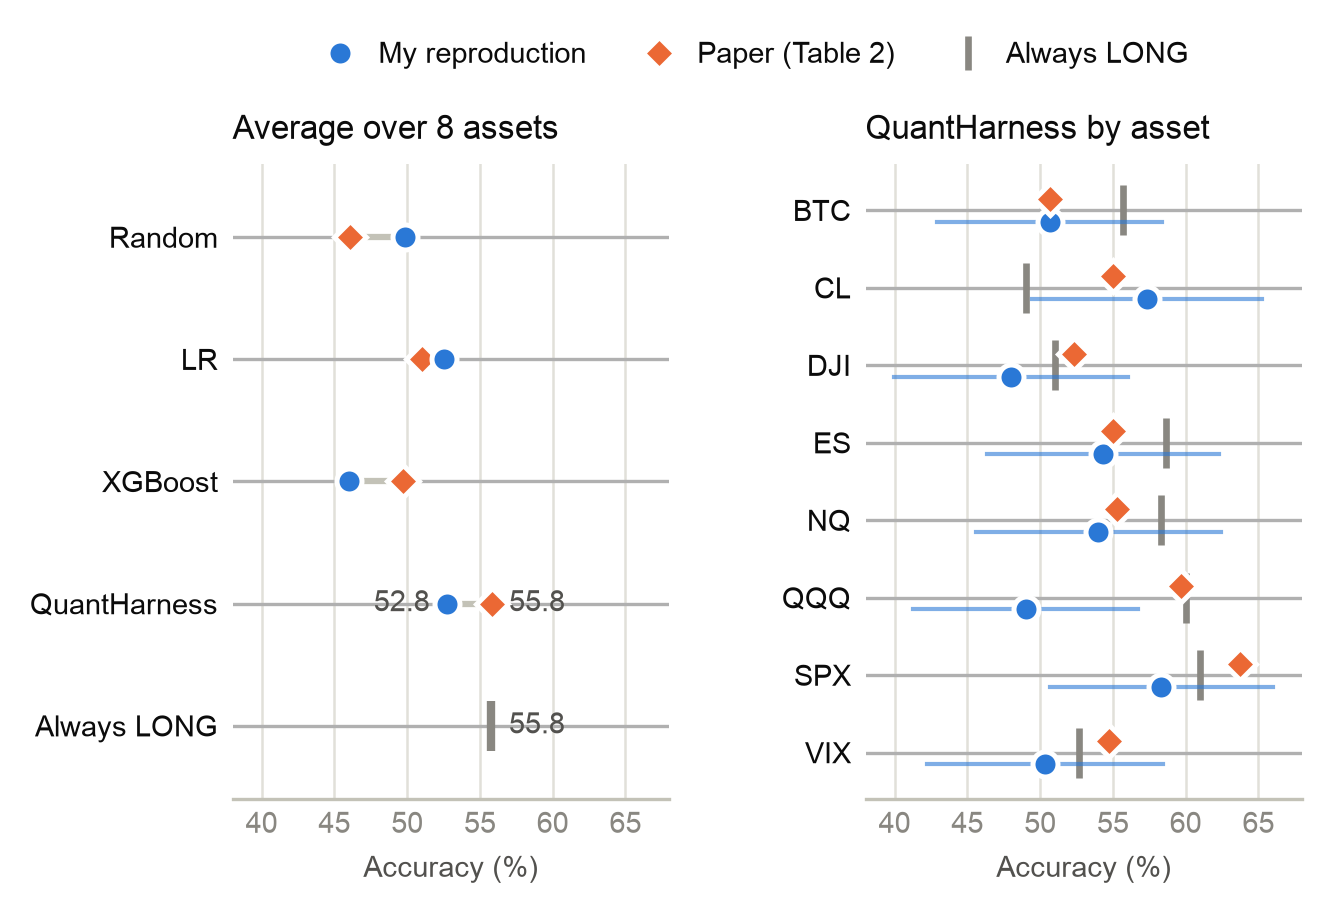
\includegraphics[width=0.86\linewidth]{accuracy_vs_paper.png}

        {\tiny 4h, 100 segments per asset. Random averaged over 100 seeds, XGBoost with a chronological split, QuantHarness mostly Gemini Flash-Lite; lines are 95\% intervals\par}

        \vspace{0.5em}
        \raggedright\footnotesize
        QuantHarness reaches \textbf{52.8\%} vs the paper's \textbf{55.8\%}, within noise on 7 of 8 assets, but it is level with LR and below always-LONG (55.8\%)
    \end{frame}


    \begin{frame}{Reproduction results: returns}
        \centering
        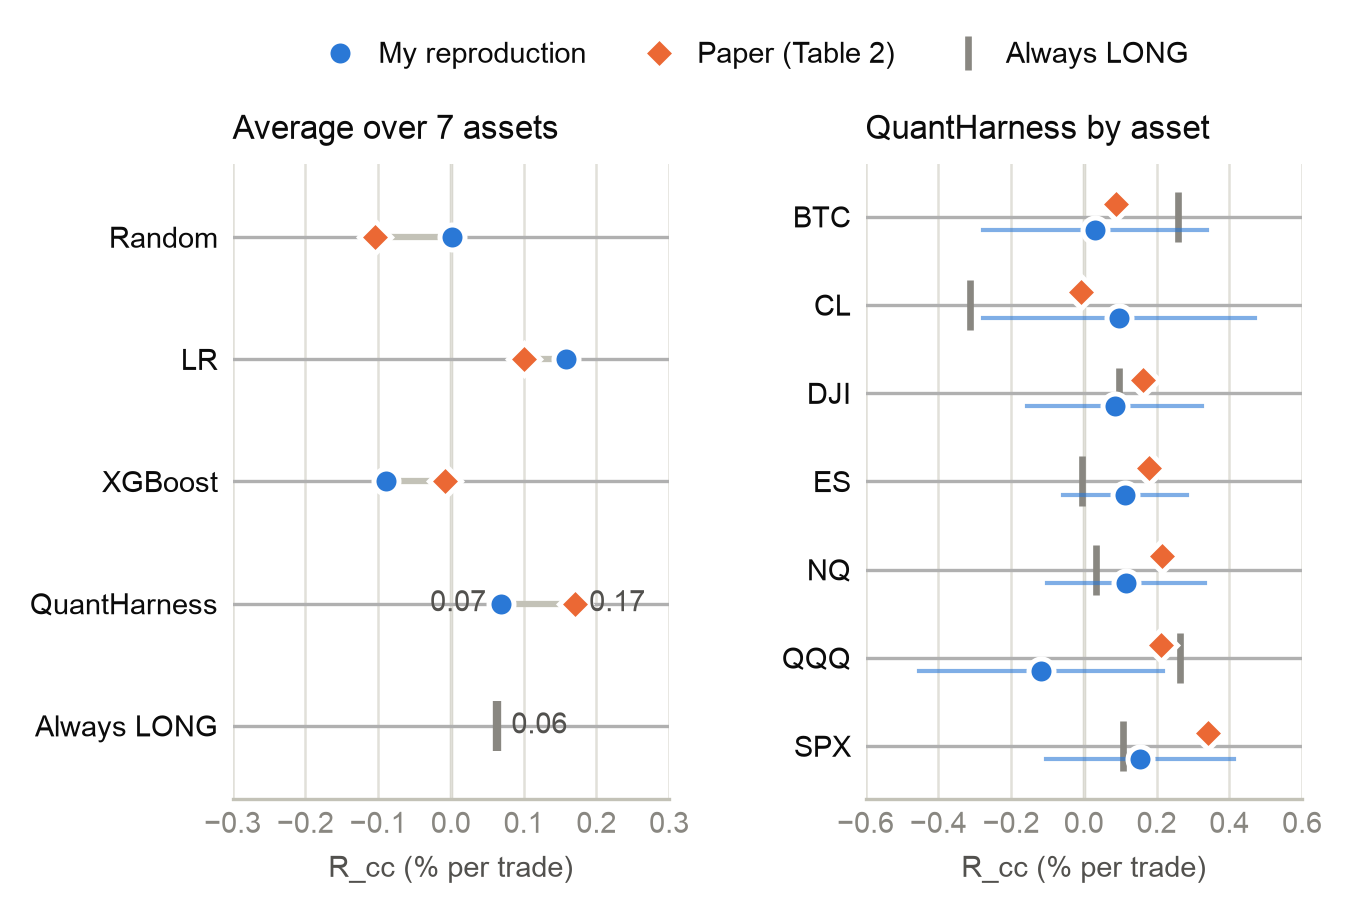
\includegraphics[width=0.82\linewidth]{returns_vs_paper.png}

        {\tiny 4h, uncapped close-to-close return over the next 3 candles. VIX is left out: its price ranges are 1.8 times the paper's; lines are 95\% intervals\par}

        \vspace{0.5em}
        \raggedright\footnotesize
        QuantHarness earns \textbf{0.07\%} per trade vs the paper's \textbf{0.17\%}: level with always-LONG, slightly below LR. $\mathcal{R}_{\max}$ and $\mathcal{R}_{\min}$ mostly track volatility
    \end{frame}


    \begin{frame}{Strengths and Limitations}
        \footnotesize
        \begin{columns}[T, onlytextwidth]
            \begin{column}{0.4\linewidth}
                \textbf{Strengths}
                \begin{itemize}
                    \item Uses only price data, so no lagging or noisy text sources
                    \item Every call comes with indicator, pattern and trend reports and a justification, so the result is interpretable
                    \item No training is required, and the code supports several LLM providers
                    \item The code and the benchmark data are open
                \end{itemize}
            \end{column}
            \begin{column}{0.56\linewidth}
                \textbf{Limitations}

                \vspace{0.4em}
                {\scriptsize\textit{Stated by the authors}\par}
                \begin{itemize}
                    \item Accuracy drops on ultra-short candles ($\approx$ 1--15 min; no numbers given)
                    \item Not exactly real-time since each decision takes several LLM calls
                \end{itemize}

                \vspace{0.4em}
                {\scriptsize\textit{Found in this reproduction}\par}
                \begin{itemize}
                    \item Does not noticeably outperform simple approaches: level with Linear Regression, below always-LONG
                    \item The paper's gains are measured against an unusually low Random baseline (below 99 of 100 seeds)
                    \item The paper and the actual code differ: no RiskAgent or stop-loss in the code, and the paper's returns are uncapped despite the caps it describes
                \end{itemize}
            \end{column}
        \end{columns}
    \end{frame}

    \begin{frame}{Suggested improvements}
        \footnotesize
        \begin{itemize}
            \setlength{\itemsep}{0.9em}
            \item \textbf{Justify the use of LLMs.} Most LLM-based approaches use text data for reasoning, while QuantHarness uses only price history. Its LLM calls cost more time and resources, yet the paper does not show that language-based reasoning beats simpler and faster numerical methods.
            \item \textbf{Use LLMs where language helps.} LLMs can be used for formulating hypotheses, generating backtesting code, interpreting diagnostic results, etc.
            \item \textbf{Keep per-candle decisions numerical.} Reading RSI, MACD and candle shapes with an LLM every hour may be an expensive and unreliable way to run what could be a simple numerical rule.
        \end{itemize}

        \vspace{1.5em}
        \colorbox{blue!8}{\parbox{\dimexpr\linewidth-2\fboxsep}{\small\raggedright\vspace{0.3em}\textbf{The main takeaway:} LLMs may be more useful for researching, designing and explaining trading strategies than for making individual trading decisions.\vspace{0.3em}}}
    \end{frame}

    % \begin{frame}[fragile]{Highlight Commands}
    %     \begin{itemize}
    %         \item \verb|\highlight|
    %         \item \verb|\highlightcap|
    %         \item \verb|\highlightcaphead|
    %         \item \verb|\highlightcapoverlay|
    %         \item \verb|\highlightcapheadoverlay|
    %     \end{itemize}
    % \end{frame}

    % \begin{frame}[plain,c]
    %     \begin{center}
    %         \Large Example Slides
    %     \end{center}
    % \end{frame}

    % \begin{frame}{Example 1 (\texttt{highlight})}
    %     \begin{align*}
    %         &x^2 - 6x + 2 \\
    %         &= \highlight[red]{x^2 - 6x + 9} - 7 \\
    %         &= \highlight[red]{(x - 3)^2} - 7
    %     \end{align*}
    % \end{frame}

    % \begin{frame}{Example 2 (\texttt{highlightcap}, \texttt{cbracket})}
    %     When we consider a Gaussian prior $p(\mathbf w | \alpha) = \mathcal N(\mathbf w | \boldsymbol 0, \alpha^{-1}\mathbf I)$,
    %     maximization of the corresponding posterior $p(\mathbf w | \boldsf{t})$ with respect to $\mathbf w$ is equivalent to the minimization of
    %     \begin{align*}
    %         \highlightcap<2->[red]{\displaystyle\frac{\beta}{2}\sum_{n=1}^N \cbracket{t_n - \mathbf w^\top\boldsymbol\phi(\mathbf x_n)}^2}{an error function}
    %         + \highlightcap<3->[blue]{\displaystyle\frac{\alpha}{2}\mathbf w^\top\mathbf w}{a quadratic regularization} \tag{3.55'}
    %     \end{align*}
    %     the minimization corresponds to (3.27) with $\lambda = \alpha/\beta$.
    % \end{frame}

    % \begin{frame}{Example 3 (\texttt{highlightcapoverlay})}
    %     For the moment, the noise precision $\beta$ as a known constant.
    %     Where the likelihood function of $t$ is defined as:
    %     %%begin novalidate
    %     \begin{align*}
    %         p(\boldsf t | \mathbf w)
    %         = \prod_{n=1}^N
    %             \highlightcapoverlay<2->{\mathcal N(t_n | \mathbf w^\top \boldsymbol\phi(\mathbf x_n), \beta^{-1})}{The exponential of a quadratic func.\ of $\mathbf w$} \tag{3.10'}
    %     \end{align*}
    %     %%end novalidate
    % \end{frame}

    % \begin{frame}{Example 4 (multi-columns)}
    %     \begin{columns}[c]
    %         \begin{column}{0.6\hsize}\centering
    %             \begin{tikzpicture}[thick,scale=0.8, every node/.style={scale=0.8}]
    %                 \node[draw, circle, minimum width=1cm] (a) at (-2, 1) {$a$};
    %                 \node[draw, circle, minimum width=1cm] (c) at (0, 0) {$c$};
    %                 \node[draw, circle, minimum width=1cm] (b) at (2, 1) {$b$};
    %                 \alt<2->{
    %                     \node[draw, circle, minimum width=1cm, fill=blue!20!white]
    %                         (d) at (0, -2) {$d$};
    %                 }{
    %                     \node[draw, circle, minimum width=1cm] (d) at (0, -2) {$d$};
    %                 }
    %                 \draw[-latex] (a) -- (c);
    %                 \draw[-latex] (b) -- (c);
    %                 \draw[-latex] (c) -- (d);
    %             \end{tikzpicture}
    %         \end{column}
    %         \begin{column}{0.4\hsize}
    %             \begin{itemize}
    %                 \item Item 1
    %                 \item Item 2
    %                 \item Item 3
    %             \end{itemize}
    %         \end{column}
    %     \end{columns}
    % \end{frame}

\end{document}
